% !TEX TS-program = pdflatex
% !TEX encoding = UTF-8 Unicode

% This is a simple template for a LaTeX document using the "article" class.
% See "book", "report", "letter" for other types of document.

\documentclass[8pt]{article} % use larger type; default would be 10pt

\usepackage[utf8]{inputenc} % set input encoding (not needed with XeLaTeX)
\usepackage{bchart}
\usepackage{longtable}
\usepackage{pgfgantt}
\usepackage{calendar} % Use the calendar.sty style
\usepackage{calc}
\usepackage{ifthen}
\usepackage{tkz-base}
\usepackage{pdfpages}
\usepackage{hyperref}
\usepackage{pgfplots}
\usepackage{tkz-kiviat,numprint,fullpage} 
\usepackage{pgfplotstable} 
\usetikzlibrary{arrows}
\usepackage{paralist} % very flexible & customisable lists (eg. enumerate/itemize, etc.)
\usepackage{dcolumn}
\usepackage{booktabs}
\usepackage{lscape}
\usepackage{pgf-pie}
\usepackage{verbatim}
\usepackage{animate}
\usepackage{sfmath}

%%% Examples of Article customizations
% These packages are optional, depending whether you want the features they provide.
% See the LaTeX Companion or other references for full information.

\usepackage{textcomp}
%\usepackage{hyperref}

%%% PAGE DIMENSIONS
\usepackage{geometry} % to change the page dimensions
\geometry{a4paper} % or letterpaper (US) or a5paper or....
% \geometry{margin=2in} % for example, change the margins to 2 inches all round
% \geometry{landscape} % set up the page for landscape
%   read geometry.pdf for detailed page layout information

\usepackage{graphicx} % support the \includegraphics command and options

% \usepackage[parfill]{parskip} % Activate to begin paragraphs with an empty line rather than an indent

%%% PACKAGES
\usepackage{booktabs} % for much better looking tables
\usepackage{array} % for better arrays (eg matrices) in maths
\usepackage{paralist} % very flexible & customisable lists (eg. enumerate/itemize, etc.)
\usepackage{verbatim} % adds environment for commenting out blocks of text & for better verbatim
\usepackage{subfig} % make it possible to include more than one captioned figure/table in a single float
% These packages are all incorporated in the memoir class to one degree or another...

%%% HEADERS & FOOTERS
\usepackage{fancyhdr} % This should be set AFTER setting up the page geometry
\pagestyle{fancy} % options: empty , plain , fancy
\renewcommand{\headrulewidth}{0pt} % customise the layout...
\lhead{}\chead{}\rhead{}
\lfoot{}\cfoot{\thepage}\rfoot{}

%%% SECTION TITLE APPEARANCE
\usepackage{sectsty}
\allsectionsfont{\sffamily\mdseries\upshape} % (See the fntguide.pdf for font help)
% (This matches ConTeXt defaults)

%%% ToC (table of contents) APPEARANCE
\usepackage[nottoc,notlof,notlot]{tocbibind} % Put the bibliography in the ToC
\usepackage[titles,subfigure]{tocloft} % Alter the style of the Table of Contents
\renewcommand{\cftsecfont}{\rmfamily\mdseries\upshape}
\renewcommand{\cftsecpagefont}{\rmfamily\mdseries\upshape} % No bold!

%%% END Article customizations

%%% The "real" document content comes below...

%\includegraphics[width=.2\textwidth]{Logo.png}

\title{Finance}
\author{\copyright Frederic Kerdraon}
%\date{} % Activate to display a given date or no date (if empty),
         % otherwise the current date is printed 

%\addtobeamertemplate{frametitle}{}{%
%\begin{tikzpicture}[remember picture,overlay]
%\node[anchor=north west,yshift=2pt] at (current page.north west) {\includegraphics[height=0.8cm]{Logo1}};
%\end{tikzpicture}}

\begin{document}
\maketitle
\tableofcontents

\newcounter{a}
\newcounter{b}
%----------------------------------------------------------
\newcommand{\slice}[4]{
  \pgfmathparse{0.5*#1+0.5*#2}
  \let\midangle\pgfmathresult

   slice
  \draw[thick,fill=black!10] (0,0) -- (#1:1) arc (#1:#2:1) -- cycle;

   outer label
  \node[label=\midangle:#4] at (\midangle:1) {};

   inner label
  \pgfmathparse{min((#2-#1-10)/110*(-0.3),0)}
  \let\temp\pgfmathresult
  \pgfmathparse{max(\temp,-0.5) + 0.9}
  \let\innerpos\pgfmathresult
  \node at (\midangle:\innerpos) {#3};
}

\section{Management summary}


\subsection{PnL Projections}

%Le nombre de simulations est egal au nombre d'arrangements des targets\\
%Pour 8 target, il devrait y avoir un 8! scenarios\\
%Les scenarios sont ordonnes par facilite de mise en oeuvre min(complexity, cost,etc)\\

\subsubsection{Latex Graph of the scenarios}

Initial parameters for the simulations.\\

%\begin{itemize}
%	\item {\$TotalDrift}
%	\item {\$TotalScenTox}
%	\item {\$TotalScenDebt}
%	\item {\$TotalScenCash}
%	\item {\$TotalScenToxDebt}
%	\item {\$TotalScen = 0}
ù\end{itemize}

We apply the scenarios below to see what we get after a few iterations\\

\subsubsection{Table}
The scenarios given in the table are only examples, the real scenarios are provided in the graph below
\begin{longtable}{|c|c|c|c|c|c|}
\hline
\multicolumn{6}{|c|}{Scenarios} \\
\hline
PnL; CumPnL; Tox; Debt(40%); Cash(50%); Tox-Debt(40%)
PnL & CumPnL & Tox & Debt(40\%) & Cash(50\%) & Tox-Debt(40\%)
\hline
-475;-475;-244;-263;-97;-32
-475 & -475 & -244 & -263 & -97 & -32\\
\hline
140;-335;126;87;419;549
140 & -335 & 126 & 87 & 419 & 549\\
\hline
136;-199;493;435;933;1128
136 & -199 & 493 & 435 & 933 & 1128\\
\hline
122;-77;846;769;1432;1693
122 & -77 & 846 & 769 & 1432 & 1693\\
\hline
82;5;1160;1063;1892;2218
82 & 5 & 1160 & 1063 & 1892 & 2218\\
\hline
70;75;1461;1345;2340;2731
70 & 75 & 1461 & 1345 & 2340 & 2731\\
\hline
63;139;1756;1620;2781;3237
63 & 139 & 1756 & 1620 & 2781 & 3237\\
\hline
43;182;2030;1874;3202;3722
43 & 182 & 2030 & 1874 & 3202 & 3722\\
\hline
37;219;2298;2123;3616;4202
37 & 219 & 2298 & 2123 & 3616 & 4202\\
\hline
-18;200;2510;2316;3975;4626
-18 & 200 & 2510 & 2316 & 3975 & 4626\\
\hline
\end{longtable}

All the figures need to be checked carefully by someone who knows what it's doing.
}

%\begin{itemize}
%	\item {\$Scen}
%	\item {\$Scenario reduction of Toxics by 231}
%	\item {\$Scenario reduction of the Debt by 529*0.4}
%	\item {\$Scenario reduction of the Cash by 755*.5}
%	\item {\$Scenario reduction of the Toxics and Debt by 231+529*.4}
%\end{itemize}

my @Scen = (231,529*.4,755*.5,231+529*.4,1000,700,800,950,750);\\

%\begin{itemize}
%	\item{The first simulation apply a reduction of the Toxics by 231 euros each month}
%	\item{The second scenario apply a reduction of the debt by 40 percent of the 529}
%	\item{The third one divide the amount of cash spent by 50 percent}
%	\item{The fourth one cumulate the reduction of the toxics by 231 euros with the amount of cash spent reduced by 50 percent}
%	\item{The fifth one is a reduction of 1000 euros each month}
%	\item{The fifth one is a reduction of 700 euros each month}
%	\item{The fifth one is a reduction of 800 euros each month}
%	\item{The fifth one is a reduction of 950 euros each month}
%	\item{The fifth one is a reduction of 750 euros each month}
%\end{itemize}

On the graph we can notice that all the scenarios are positive, as they were built to show how to maximize profit
just by managing the charge, and especially useless charges.\\

%my $Drift = $row->{Drift};
%$NewDrift = $Drift + $NewDrift;
%my $KDrift = $Drift/$Unit;
%$TotalDrift = $TotalDrift + $Drift;
%$TotalScenTox = $TotalDrift + $ScenToxics*$Count;
%$TotalScenDebt = $TotalDrift + $ScenDebt*$Count;
%$TotalScenCash = $TotalDrift + $ScenCash*$Count;
%$TotalScenToxDebt = $TotalDrift + $ScenToxDebt*$Count;

%\setlength{\unitlength}{1cm}
\begin{picture}(12,11)(0,0)
\put(0,0){\vector(1,0){12.1}}
\put(12,-.35){$Month$}
\put(0,-6){\vector(0,1){12}}
\put(0,6.5){\makebox(0,0){$PnL$)}}
\put( -0.5,1){$1$}
\put( -0.5,2){$2$}
\put( -0.5,3){$3$}
\put( -0.5,4){$4$}
\put( -0.5,5){$5$}
\put( -0.5,6){$6$}
\put( -0.5,-1){$-1$}
\put( -0.5,-2){$-2$}
\put( -0.5,-3){$-3$}
\put( -0.5,-4){$-4$}
\put( -0.5,-5){$-5$}
\put( -0.5,-6){$-6$}
\qbezier(0.0,0.0)(1.2384,0.0)(2.0,2.7622)
\linethickness{.090mm}
\put( 0,6){$1$}
\put( 0,0.472810){\line(2,0){.2}}
\put( 0,0){\line(0,1){0.472810}}
\put( 0.2,0){\line(0,1){0.472810}}
\put( 0,0.572810){$Scen0$}
\put( 0,0.703810){\line(2,0){.5}}
\put( 0,0){\line(0,1){0.703810}}
\put( 0.5,0){\line(0,1){0.703810}}
\put( 0,0.684410){\line(2,0){.5}}
\put( 0,0){\line(0,1){0.684410}}
\put( 0.5,0){\line(0,1){0.684410}}
\put( 1,6){$2$}
\put( 1,-0.002590){\line(2,0){.2}}
\put( 1,-0.002590){\line(0,1){0.002590}}
\put( 1.2,-0.002590){\line(0,1){0.002590}}
\put( 1,-0.302590){$Scen0$}
\put( 1,0.459410){\line(2,0){.5}}
\put( 1,0){\line(0,1){0.459410}}
\put( 1.5,0){\line(0,1){0.459410}}
\put( 1,0.420610){\line(2,0){.5}}
\put( 1,0){\line(0,1){0.420610}}
\put( 1.5,0){\line(0,1){0.420610}}
\end{picture}

%\begin{tikzpicture}[thick, scale=1]
\begin{axis}[
title={Kapital over time},
ybar, axis on top,
title={PnL over the months},
height=8cm, width=15.5cm,
bar width=0.4cm,
ymajorgrids, tick align=inside,
major grid style={draw=white},
enlarge y limits={value=.1,upper},
axis x line*=bottom,
axis y line*=right,
y axis line style={opacity=0},
tickwidth=0pt,
enlarge x limits=true,
legend style={
at={(0.5,-0.2)},
anchor=north,
legend columns=-1,
/tikz/every even column/.append style={column sep=0.5cm}
},
ylabel={Percentage (\%)},
symbolic x coords={
xlabel={Time [Days]},
ylabel={Kapital [euro]},
ymin=0,ymax=0,
xtick=data,
nodes near coords={
\pgfmathprintnumber[precision=0]{\pgfplotspointmeta}
}
]
\addplot [draw=none, fill=black!50] coordinates {
};
\addplot [draw=none, fill=black!100] coordinates {
};
\addplot [draw=none, fill=red!100] coordinates {
};

\legend{Income,Charges,CashBalance}
\end{axis}
\end{tikzpicture}

%{\footnotesize
%BarPlotPnl
%}
\subsubsection{PnL}
%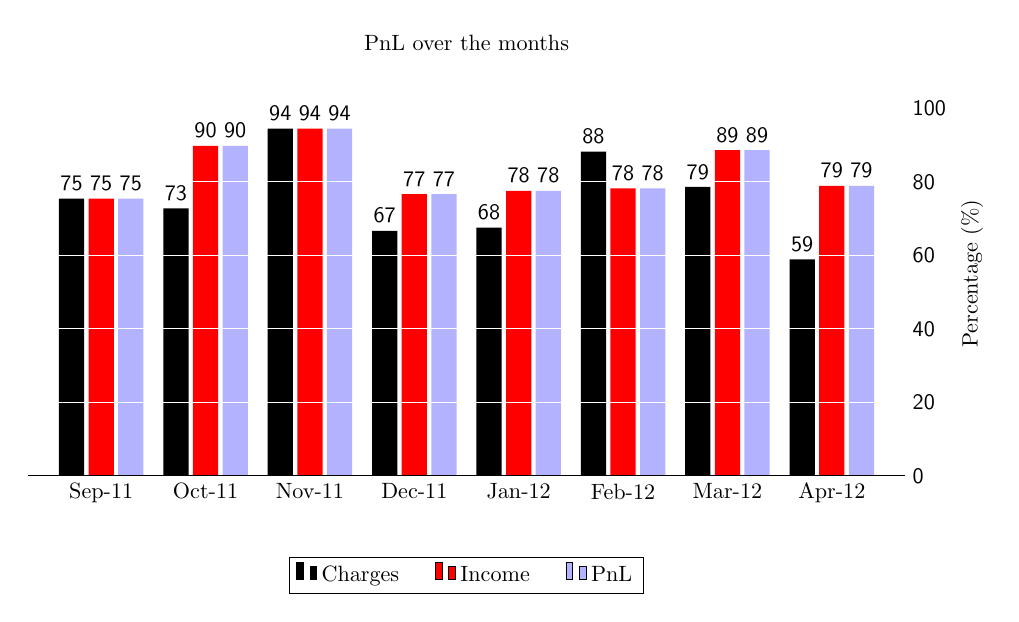
\begin{tikzpicture}[scale=0.8]
  \centering
  \begin{axis}[
        ybar, axis on top,
        title={PnL over the months},
        height=8cm, width=15.5cm,
        bar width=0.4cm,
        ymajorgrids, tick align=inside,
        major grid style={draw=white},
        enlarge y limits={value=.1,upper},
        ymin=0, ymax=100,
        axis x line*=bottom,
        axis y line*=right,
        y axis line style={opacity=0},
        tickwidth=0pt,
        enlarge x limits=true,
        legend style={
            at={(0.5,-0.2)},
            anchor=north,
            legend columns=-1,
            /tikz/every even column/.append style={column sep=0.5cm}
        },
        ylabel={Percentage (\%)},
        symbolic x coords={
           Sep-11,Oct-11,Nov-11,Dec-11,
           Jan-12,Feb-12,
           Mar-12,
          Apr-12},
       xtick=data,
       nodes near coords={
        \pgfmathprintnumber[precision=0]{\pgfplotspointmeta}
       }
    ]
    \addplot [draw=none, fill=black!100] coordinates {
      (Sep-11,75.4064)
      (Oct-11, 72.7961) 
      (Nov-11,94.4597)
      (Dec-11,66.6786) 
      (Jan-12,67.5600) 
      (Feb-12,88.2339)
      (Mar-12,78.6138) 
      (Apr-12,58.9129) };
   \addplot [draw=none,fill=red!100] coordinates {
      (Sep-11,75.4064)
      (Oct-11, 89.7961) 
      (Nov-11,94.4597)
      (Dec-11,76.6786) 
      (Jan-12,77.5600) 
      (Feb-12,78.2339)
      (Mar-12,88.6138) 
      (Apr-12,78.9129) };
   \addplot [draw=none, fill=blue!30] coordinates {
      (Sep-11,75.4064)
      (Oct-11, 89.7961) 
      (Nov-11,94.4597)
      (Dec-11,76.6786) 
      (Jan-12,77.5600) 
      (Feb-12,78.2339)
      (Mar-12,88.6138) 
      (Apr-12,78.9129) };

    \legend{Charges,Income,PnL}
  \end{axis}
  \end{tikzpicture}


\begin{tikzpicture}[thick, scale=1]
\begin{axis}[
title={Kapital over time},
ybar, axis on top,
title={PnL over the months},
height=8cm, width=15.5cm,
bar width=0.4cm,
ymajorgrids, tick align=inside,
major grid style={draw=white},
enlarge y limits={value=.1,upper},
axis x line*=bottom,
axis y line*=right,
y axis line style={opacity=0},
tickwidth=0pt,
enlarge x limits=true,
legend style={
at={(0.5,-0.2)},
anchor=north,
legend columns=-1,
/tikz/every even column/.append style={column sep=0.5cm}
},
ylabel={Percentage (\%)},
symbolic x coords={
xlabel={Time [Days]},
ylabel={Kapital [euro]},
ymin=0,ymax=0,
xtick=data,
nodes near coords={
\pgfmathprintnumber[precision=0]{\pgfplotspointmeta}
}
]
\addplot [draw=none, fill=black!50] coordinates {
};
\addplot [draw=none, fill=black!100] coordinates {
};
\addplot [draw=none, fill=red!100] coordinates {
};

\legend{Income,Charges,CashBalance}
\end{axis}
\end{tikzpicture}

\subsubsection{Kapital}
%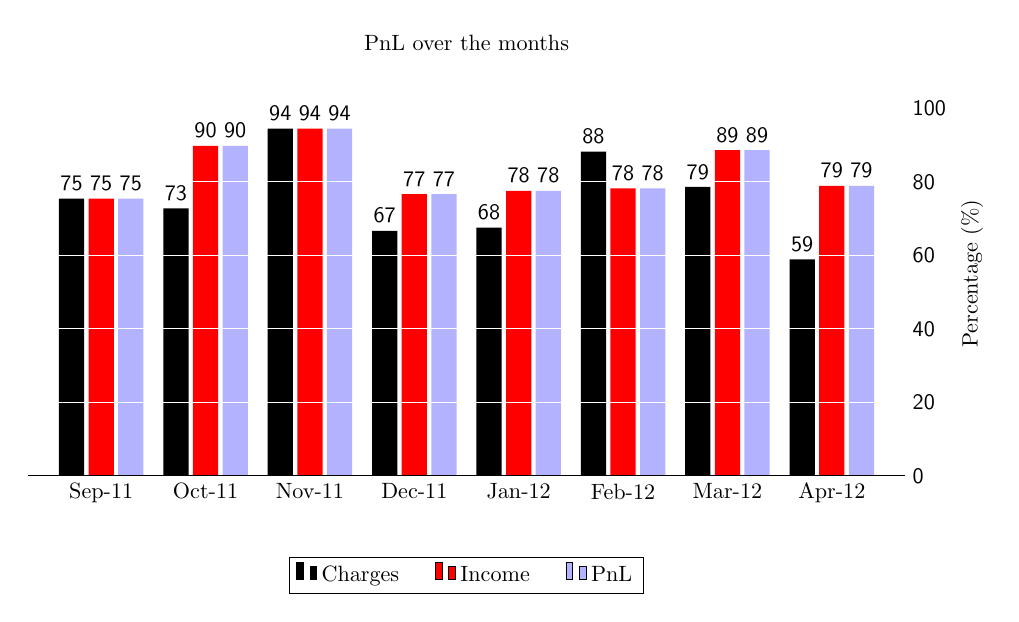
\begin{tikzpicture}[scale=0.8]
  \centering
  \begin{axis}[
        ybar, axis on top,
        title={PnL over the months},
        height=8cm, width=15.5cm,
        bar width=0.4cm,
        ymajorgrids, tick align=inside,
        major grid style={draw=white},
        enlarge y limits={value=.1,upper},
        ymin=0, ymax=100,
        axis x line*=bottom,
        axis y line*=right,
        y axis line style={opacity=0},
        tickwidth=0pt,
        enlarge x limits=true,
        legend style={
            at={(0.5,-0.2)},
            anchor=north,
            legend columns=-1,
            /tikz/every even column/.append style={column sep=0.5cm}
        },
        ylabel={Percentage (\%)},
        symbolic x coords={
           Sep-11,Oct-11,Nov-11,Dec-11,
           Jan-12,Feb-12,
           Mar-12,
          Apr-12},
       xtick=data,
       nodes near coords={
        \pgfmathprintnumber[precision=0]{\pgfplotspointmeta}
       }
    ]
    \addplot [draw=none, fill=black!100] coordinates {
      (Sep-11,75.4064)
      (Oct-11, 72.7961) 
      (Nov-11,94.4597)
      (Dec-11,66.6786) 
      (Jan-12,67.5600) 
      (Feb-12,88.2339)
      (Mar-12,78.6138) 
      (Apr-12,58.9129) };
   \addplot [draw=none,fill=red!100] coordinates {
      (Sep-11,75.4064)
      (Oct-11, 89.7961) 
      (Nov-11,94.4597)
      (Dec-11,76.6786) 
      (Jan-12,77.5600) 
      (Feb-12,78.2339)
      (Mar-12,88.6138) 
      (Apr-12,78.9129) };
   \addplot [draw=none, fill=blue!30] coordinates {
      (Sep-11,75.4064)
      (Oct-11, 89.7961) 
      (Nov-11,94.4597)
      (Dec-11,76.6786) 
      (Jan-12,77.5600) 
      (Feb-12,78.2339)
      (Mar-12,88.6138) 
      (Apr-12,78.9129) };

    \legend{Charges,Income,PnL}
  \end{axis}
  \end{tikzpicture}


\begin{tikzpicture}[thick, scale=1]
\begin{axis}[
title={Kapital over time},
ybar, axis on top,
title={PnL over the months},
height=8cm, width=15.5cm,
bar width=0.4cm,
ymajorgrids, tick align=inside,
major grid style={draw=white},
enlarge y limits={value=.1,upper},
axis x line*=bottom,
axis y line*=right,
y axis line style={opacity=0},
tickwidth=0pt,
enlarge x limits=true,
legend style={
at={(0.5,-0.2)},
anchor=north,
legend columns=-1,
/tikz/every even column/.append style={column sep=0.5cm}
},
ylabel={Percentage (\%)},
symbolic x coords={
xlabel={Time [Days]},
ylabel={Kapital [euro]},
ymin=-11.02157,ymax=21.77043,
Jan-18,Feb-18,Mar-18,Apr-18,May-18,Jun-18,Jul-18,Aug-18,Sep-18,Oct-18,Nov-18,xtick=data,
nodes near coords={
\pgfmathprintnumber[precision=0]{\pgfplotspointmeta}
}
]
\addplot [draw=none, fill=red!100] coordinates {
(Jan-18,-83.8994)
(Feb-18,-46.97312)
(Mar-18,-52.03197)
(Apr-18,-52.81598)
(May-18,-96.81726)
(Jun-18,-87.10997)
(Jul-18,-88.51826)
(Aug-18,-113.91554)
(Sep-18,-107.10126)
(Oct-18,-141.31811)
(Nov-18,-50.46756)
};
\addplot [draw=none, fill=black!100] coordinates {
(Jan-18,468.16)
(Feb-18,374.528)
(Mar-18,491.568)
(Apr-18,327.712)
(May-18,421.344)
(Jun-18,491.568)
(Jul-18,421.344)
(Aug-18,514.976)
(Sep-18,421.344)
(Oct-18,538.384)
(Nov-18,187.264)
};
\addplot [draw=none, fill=black!50] coordinates {
(Jan-18,654.9914)
(Feb-18,523.99312)
(Mar-18,687.74097)
(Apr-18,458.49398)
(May-18,589.49226)
(Jun-18,687.74097)
(Jul-18,589.49226)
(Aug-18,720.49054)
(Sep-18,589.49226)
(Oct-18,753.24011)
(Nov-18,261.99656)
};

\legend{Assets,Liabilities,Kapital}
\end{axis}
\end{tikzpicture}

%\subsubsection{Plot of an example}
%\includegraphics[scale=0.3]{Finance.png}}

%tableae.dat\\
%file.dat\\
%immigration.dat\\
%finance.dat\\
%charges.dat\\
%article_contourtmp0.dat\\
%Surface4_contourtmp0.dat\\
%pgfplots_scatterdata4.dat\\
%assets.dat\\
%chargesKiviat.dat\\
%resourcesKiviat.dat\\

%\subsubsection{Latex example}
%\input{parabola-plot}

%\subsubsection{Latex example}
%\input{tikzdevice-demo}

%\subsubsection{Latex example}
%\input{TimeTable}

%\subsubsection{Latex example}
%\input{Torn Paper}

%\subsubsection{Latex example}
%\input{Weather Table}

%\subsubsection{Latex example}
%

\documentclass[a5paper]{article}

% Requires PGF >=  1.09
% Note:
%   This example works only with pdftex >= 1.30.0
%   You have to run pdftex on the example twice!
\usepackage{amsmath}
\usepackage{tikz}

\begin{document}
\thispagestyle{empty}

Lorem ipsum dolor sit amet, consectetuer adipiscing elit. Donec luctus 
mollis nisl. Nullam tempor, diam non tincidunt tincidunt, nunc tortor 
elementum odio, nec iaculis urna leo a eros. Lorem ipsum dolor sit amet,
consectetuer adipiscing elit. Sed elit elit, pellentesque et, 
sollicitudin a, imperdiet eget, tellus. Vestibulum et sapien. Maecenas 
libero. Vivamus vel metus in ipsum ultricies commodo. Donec quam. Fusce 
arcu. In est felis, sagittis vitae, vehicula ut, tristique vitae, eros. 
Mauris ut lorem vel risus posuere elementum. Quisque volutpat ornare lorem. 
Integer porta.
\begin{multline}\label{eq:steeringfull}
    \begin{bmatrix}
        m-Y_{\dot{v}} & Y_{\dot{r}} & 0\\
        -N_{\dot{v}} & I_z-N_{\dot{r}} & 0\\
        0 & 0 & 1
    \end{bmatrix}
    \begin{bmatrix}
        \dot{v} \\ \dot{r}\\ \dot{\psi}
    \end{bmatrix}\\ +
    \begin{bmatrix}
        -Y_v & -Y_r+mu_0\\
        -N_v & -N_r & 0\\
        0 & -1 & 0
    \end{bmatrix}
    \begin{bmatrix}
        v \\ r \\ \psi
    \end{bmatrix} =
    \begin{bmatrix}
        Y_\delta \\ N_\delta \\ 0
    \end{bmatrix}\delta_r
\end{multline}

Donec ut neque vel leo sagittis tristique. Cras et justo. Mauris lorem 
purus, sagittis eu, consectetuer et, lacinia et, augue. Ut in velit in 
diam semper rutrum. Nunc rhoncus. Cras tincidunt. Aenean nec quam. In commodo
sem ac nulla. Donec fermentum metus non nisl sagittis sagittis. Vestibulum 
sit amet nunc. Vivamus dapibus congue purus. Quisque arcu tellus, 
pellentesque ac, tincidunt lobortis, commodo ac, purus.


% Start of the interesting part
% If you place the code at the beginning of the page, the image will be
% put behind the text.
%
% The overlay option removes the picture from the ordinary page flow. 
\begin{tikzpicture}[remember picture, overlay]
    \node[inner sep=0pt] at (current page.center) {%
        \includegraphics[width=\paperwidth,height=\paperheight]{007}%
    };%
\end{tikzpicture}


\end{document}



%\includepdf[pages={1}]{stockchart.pdf}
%\includepdf[pages={1}]{friedberg.pdf}
%\subsubsection{Surface}
%\begin{tikzpicture}
\begin{axis}
\addplot[color=red]{exp(x)};
\end{axis}
\end{tikzpicture}
%Here ends the furst plot
\hskip 5pt
%Here begins the 3d plot
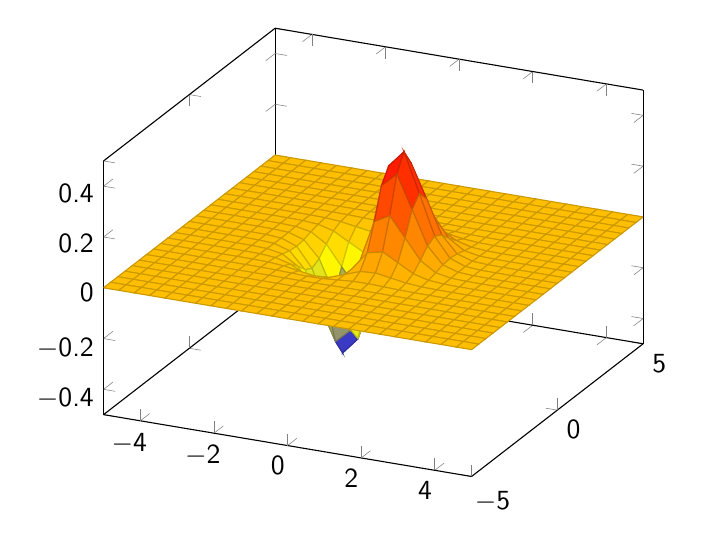
\begin{tikzpicture}
\begin{axis}
\addplot3[
    surf,
]
{exp(-x^2-y^2)*x};
\end{axis}
\end{tikzpicture}


%\subsubsection{Gaussian Curve}
%\includepdf[pages={1}]{GaussianCurve.pdf}
%\input{GaussianCurve}
%Was removed because very uncomplete...

%\subsubsection{Parabola}
%This I beleive should be the logo for the finance document, so that every doc has it's logo now :-)\\
%\includepdf[pages={1}]{parabola-plotpdf}
%\input{parabola-plot}

%\subsubsection{Weather}
%\includepdf[pages={1}]{WeatherTable.pdf}
%\input{WeatherTable2}

%\subsubsection{Map Of The Charges}
%\includepdf[pages={1}]{MapOfTheCharges.pdf}
%%\centering

%\begin{tikzpicture}[scale=0.5]
%\pie{13/A, 27/B, 30/C, 35/D}
%\end{tikzpicture}
%
\hspace{1cm}
%
%\begin{tikzpicture}[scale=0.5]
%  \pie[polar]{10/A, 20/B, 30/C, 40/D}
%\end{tikzpicture}

%\vspace{2cm}

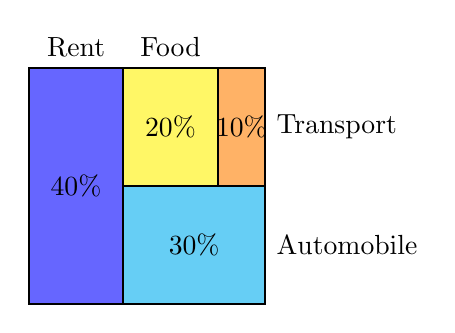
\begin{tikzpicture}[scale=0.5]
  \pie[square]{40/Rent, 30/Automobile, 20/Food, 10/Transport}
\end{tikzpicture}
%
\hspace{1cm}
%
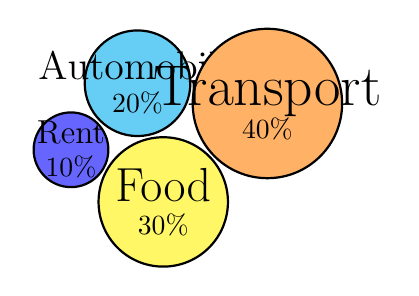
\begin{tikzpicture}[scale=0.5]
  \pie[cloud, text=inside, scale font]{10/Rent, 20/Automobile, 30/Food, 40/Transport}
\end{tikzpicture}


\subsubsection{Table}
The scenarios given in the table are only examples, the real scenarios are provided in the graph below
\begin{longtable}{|c|c|c|c|c|c|}
\hline
\multicolumn{6}{|c|}{Scenarios} \\
\hline
PnL; CumPnL; Tox; Debt(40%); Cash(50%); Tox-Debt(40%)
PnL & CumPnL & Tox & Debt(40\%) & Cash(50\%) & Tox-Debt(40\%)
\hline
-475;-475;-244;-263;-97;-32
-475 & -475 & -244 & -263 & -97 & -32\\
\hline
140;-335;126;87;419;549
140 & -335 & 126 & 87 & 419 & 549\\
\hline
136;-199;493;435;933;1128
136 & -199 & 493 & 435 & 933 & 1128\\
\hline
122;-77;846;769;1432;1693
122 & -77 & 846 & 769 & 1432 & 1693\\
\hline
82;5;1160;1063;1892;2218
82 & 5 & 1160 & 1063 & 1892 & 2218\\
\hline
70;75;1461;1345;2340;2731
70 & 75 & 1461 & 1345 & 2340 & 2731\\
\hline
63;139;1756;1620;2781;3237
63 & 139 & 1756 & 1620 & 2781 & 3237\\
\hline
43;182;2030;1874;3202;3722
43 & 182 & 2030 & 1874 & 3202 & 3722\\
\hline
37;219;2298;2123;3616;4202
37 & 219 & 2298 & 2123 & 3616 & 4202\\
\hline
-18;200;2510;2316;3975;4626
-18 & 200 & 2510 & 2316 & 3975 & 4626\\
\hline
\end{longtable}

All the figures need to be checked carefully by someone who knows what it's doing.
}

\subsection{History and extrapolations}

\subsubsection{Kapital curve}
Kapital trend,Assets trend,Liabilities trend,Leverage trend\\
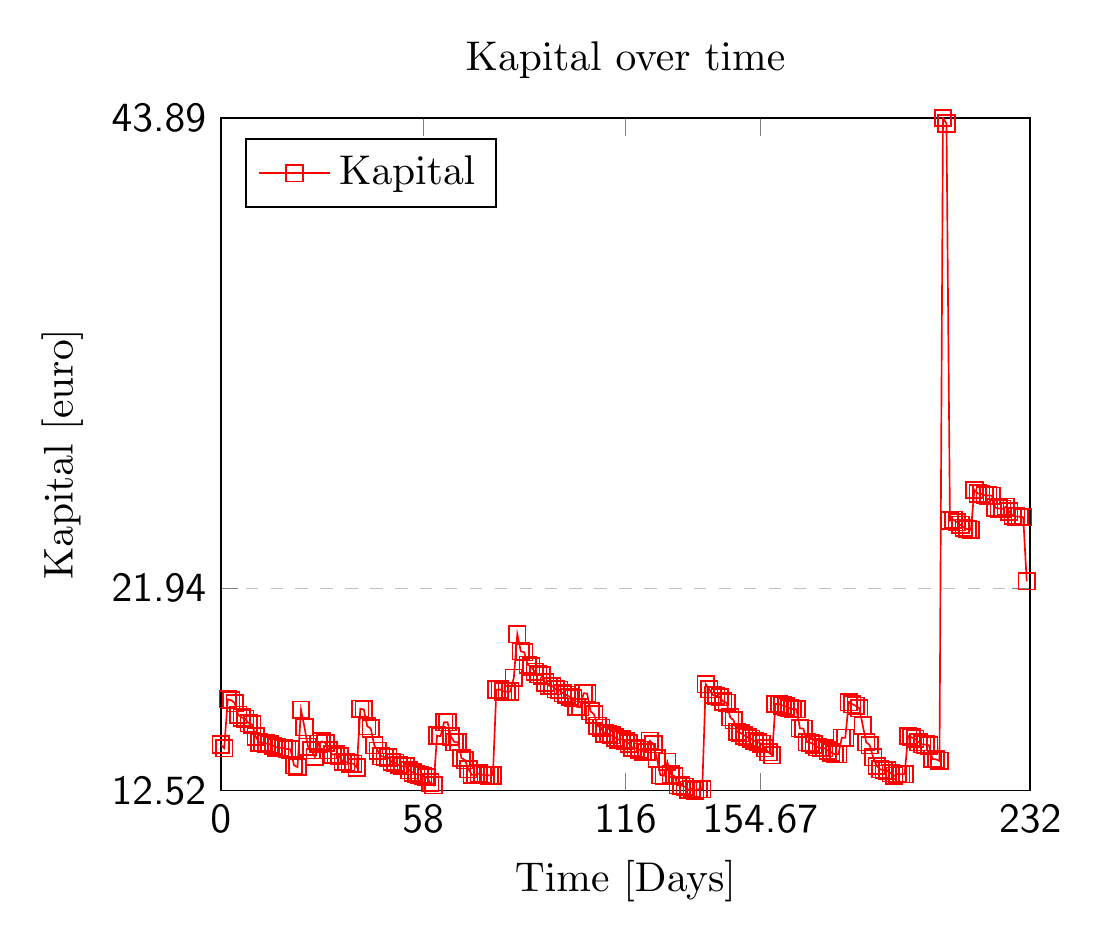
\begin{tikzpicture}[thick, scale=1.5]
\begin{axis}[
title={Kapital over time},
xlabel={Time [Days]},
ylabel={Kapital [euro]},
xmin=0,xmax=232,
ymin=12.515,ymax=43.885,
xtick={0,58,116,154.666666666667,232},
ytick={12.515,6.2575,0,21.9425,43.885},
legend pos=north west,
ymajorgrids=true,
grid style=dashed,
]
\addplot[
color=red,
mark=square,
]
coordinates {
(0,14.653)(1,14.488)(2,16.766)(3,16.726)(4,16.589)(5,16.042)(6,15.923)(7,15.856)(8,15.651)(9,15.59)(10,15.037)(11,14.751)(12,14.733)(13,14.708)(14,14.673)(15,14.603)(16,14.525)(17,14.505)(18,14.491)(19,14.448)(20,14.428)(21,13.693)(22,13.609)(23,16.276)(24,15.46)(25,14.556)(26,14.398)(27,14.076)(28,14.698)(29,14.803)(30,14.729)(31,14.39)(32,14.191)(33,14.191)(34,14.111)(35,13.856)(36,13.832)(37,13.772)(38,13.763)(39,13.586)(40,16.325)(41,16.298)(42,15.507)(43,15.406)(44,14.628)(45,14.37)(46,14.116)(47,14.08)(48,14.057)(49,13.846)(50,13.802)(51,13.702)(52,13.647)(53,13.647)(54,13.453)(55,13.357)(56,13.277)(57,13.252)(58,13.202)(59,13.142)(60,12.888)(61,12.761)(62,15.079)(63,15.046)(64,15.696)(65,15.696)(66,15.026)(67,14.764)(68,14.76)(69,14.029)(70,13.931)(71,13.508)(72,13.24)(73,13.242)(74,13.306)(75,13.248)(76,13.225)(77,13.219)(78,13.219)(79,17.219)(80,17.229)(81,17.137)(82,17.123)(83,17.128)(84,17.778)(85,19.812)(86,19.007)(87,18.958)(88,18.381)(89,18.293)(90,18.054)(91,17.934)(92,17.874)(93,17.549)(94,17.405)(95,17.385)(96,17.235)(97,17.215)(98,17.057)(99,16.977)(100,16.876)(101,16.812)(102,16.417)(103,16.402)(104,17.052)(105,17.036)(106,16.207)(107,16.061)(108,15.528)(109,15.433)(110,15.175)(111,15.159)(112,15.086)(113,14.99)(114,14.89)(115,14.89)(116,14.81)(117,14.706)(118,14.499)(119,14.487)(120,14.412)(121,14.326)(122,14.308)(123,14.829)(124,14.678)(125,14.008)(126,13.233)(127,13.205)(128,13.847)(129,13.258)(130,13.19)(131,12.757)(132,12.747)(133,12.687)(134,12.551)(135,12.597)(136,12.515)(137,12.573)(138,12.573)(139,17.473)(140,17.239)(141,16.974)(142,16.928)(143,16.867)(144,16.663)(145,16.602)(146,15.929)(147,15.785)(148,15.256)(149,15.194)(150,15.083)(151,15.007)(152,14.917)(153,14.827)(154,14.765)(155,14.685)(156,14.484)(157,14.295)(158,14.162)(159,16.547)(160,16.546)(161,16.481)(162,16.43)(163,16.35)(164,16.308)(165,16.299)(166,15.415)(167,15.399)(168,14.772)(169,14.742)(170,14.662)(171,14.53)(172,14.495)(173,14.49)(174,14.384)(175,14.291)(176,14.207)(177,14.199)(178,14.977)(179,14.967)(180,16.639)(181,16.539)(182,16.463)(183,16.357)(184,15.551)(185,14.762)(186,14.627)(187,14.066)(188,13.657)(189,13.499)(190,13.466)(191,13.448)(192,13.327)(193,13.196)(194,13.287)(195,13.272)(196,13.272)(197,15.056)(198,14.996)(199,14.919)(200,14.767)(201,14.666)(202,14.654)(203,14.618)(204,13.984)(205,13.966)(206,13.893)(207,43.885)(208,43.629)(209,25.102)(210,25.145)(211,25.035)(212,24.904)(213,24.775)(214,24.702)(215,24.668)(216,26.531)(217,26.371)(218,26.353)(219,26.283)(220,26.272)(221,26.267)(222,25.715)(223,25.667)(224,25.65)(225,25.749)(226,25.524)(227,25.32)(228,25.3)(229,25.283)(230,25.262)(231,22.271)
};
\legend{Kapital}
\end{axis}
\end{tikzpicture}


\subsubsection{PnL curve}
%\input{pnlCurve}
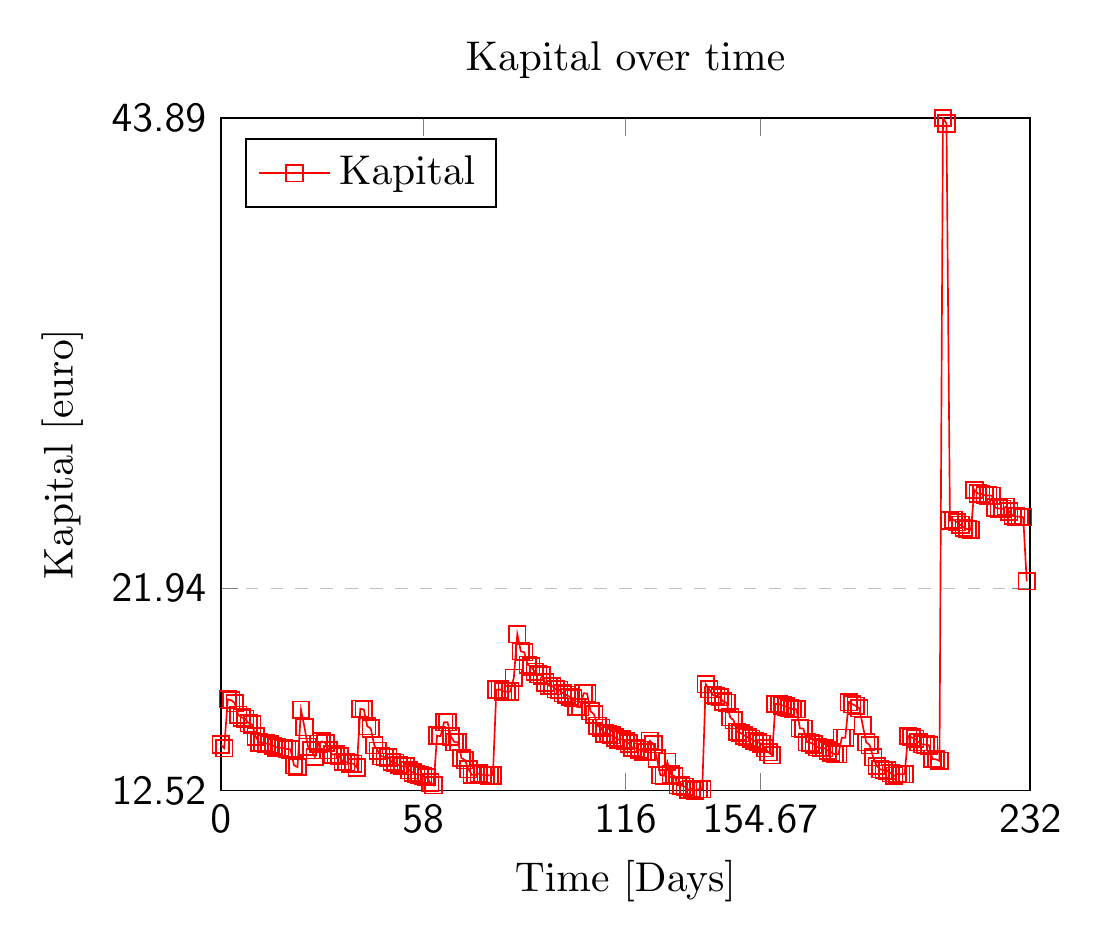
\begin{tikzpicture}[thick, scale=1.5]
\begin{axis}[
title={Kapital over time},
xlabel={Time [Days]},
ylabel={Kapital [euro]},
xmin=0,xmax=232,
ymin=12.515,ymax=43.885,
xtick={0,58,116,154.666666666667,232},
ytick={12.515,6.2575,0,21.9425,43.885},
legend pos=north west,
ymajorgrids=true,
grid style=dashed,
]
\addplot[
color=red,
mark=square,
]
coordinates {
(0,14.653)(1,14.488)(2,16.766)(3,16.726)(4,16.589)(5,16.042)(6,15.923)(7,15.856)(8,15.651)(9,15.59)(10,15.037)(11,14.751)(12,14.733)(13,14.708)(14,14.673)(15,14.603)(16,14.525)(17,14.505)(18,14.491)(19,14.448)(20,14.428)(21,13.693)(22,13.609)(23,16.276)(24,15.46)(25,14.556)(26,14.398)(27,14.076)(28,14.698)(29,14.803)(30,14.729)(31,14.39)(32,14.191)(33,14.191)(34,14.111)(35,13.856)(36,13.832)(37,13.772)(38,13.763)(39,13.586)(40,16.325)(41,16.298)(42,15.507)(43,15.406)(44,14.628)(45,14.37)(46,14.116)(47,14.08)(48,14.057)(49,13.846)(50,13.802)(51,13.702)(52,13.647)(53,13.647)(54,13.453)(55,13.357)(56,13.277)(57,13.252)(58,13.202)(59,13.142)(60,12.888)(61,12.761)(62,15.079)(63,15.046)(64,15.696)(65,15.696)(66,15.026)(67,14.764)(68,14.76)(69,14.029)(70,13.931)(71,13.508)(72,13.24)(73,13.242)(74,13.306)(75,13.248)(76,13.225)(77,13.219)(78,13.219)(79,17.219)(80,17.229)(81,17.137)(82,17.123)(83,17.128)(84,17.778)(85,19.812)(86,19.007)(87,18.958)(88,18.381)(89,18.293)(90,18.054)(91,17.934)(92,17.874)(93,17.549)(94,17.405)(95,17.385)(96,17.235)(97,17.215)(98,17.057)(99,16.977)(100,16.876)(101,16.812)(102,16.417)(103,16.402)(104,17.052)(105,17.036)(106,16.207)(107,16.061)(108,15.528)(109,15.433)(110,15.175)(111,15.159)(112,15.086)(113,14.99)(114,14.89)(115,14.89)(116,14.81)(117,14.706)(118,14.499)(119,14.487)(120,14.412)(121,14.326)(122,14.308)(123,14.829)(124,14.678)(125,14.008)(126,13.233)(127,13.205)(128,13.847)(129,13.258)(130,13.19)(131,12.757)(132,12.747)(133,12.687)(134,12.551)(135,12.597)(136,12.515)(137,12.573)(138,12.573)(139,17.473)(140,17.239)(141,16.974)(142,16.928)(143,16.867)(144,16.663)(145,16.602)(146,15.929)(147,15.785)(148,15.256)(149,15.194)(150,15.083)(151,15.007)(152,14.917)(153,14.827)(154,14.765)(155,14.685)(156,14.484)(157,14.295)(158,14.162)(159,16.547)(160,16.546)(161,16.481)(162,16.43)(163,16.35)(164,16.308)(165,16.299)(166,15.415)(167,15.399)(168,14.772)(169,14.742)(170,14.662)(171,14.53)(172,14.495)(173,14.49)(174,14.384)(175,14.291)(176,14.207)(177,14.199)(178,14.977)(179,14.967)(180,16.639)(181,16.539)(182,16.463)(183,16.357)(184,15.551)(185,14.762)(186,14.627)(187,14.066)(188,13.657)(189,13.499)(190,13.466)(191,13.448)(192,13.327)(193,13.196)(194,13.287)(195,13.272)(196,13.272)(197,15.056)(198,14.996)(199,14.919)(200,14.767)(201,14.666)(202,14.654)(203,14.618)(204,13.984)(205,13.966)(206,13.893)(207,43.885)(208,43.629)(209,25.102)(210,25.145)(211,25.035)(212,24.904)(213,24.775)(214,24.702)(215,24.668)(216,26.531)(217,26.371)(218,26.353)(219,26.283)(220,26.272)(221,26.267)(222,25.715)(223,25.667)(224,25.65)(225,25.749)(226,25.524)(227,25.32)(228,25.3)(229,25.283)(230,25.262)(231,22.271)
};
\legend{Kapital}
\end{axis}
\end{tikzpicture}


%\subsubsection{Cash curve}
%Funny cashflow/kapital superior to percent\\
%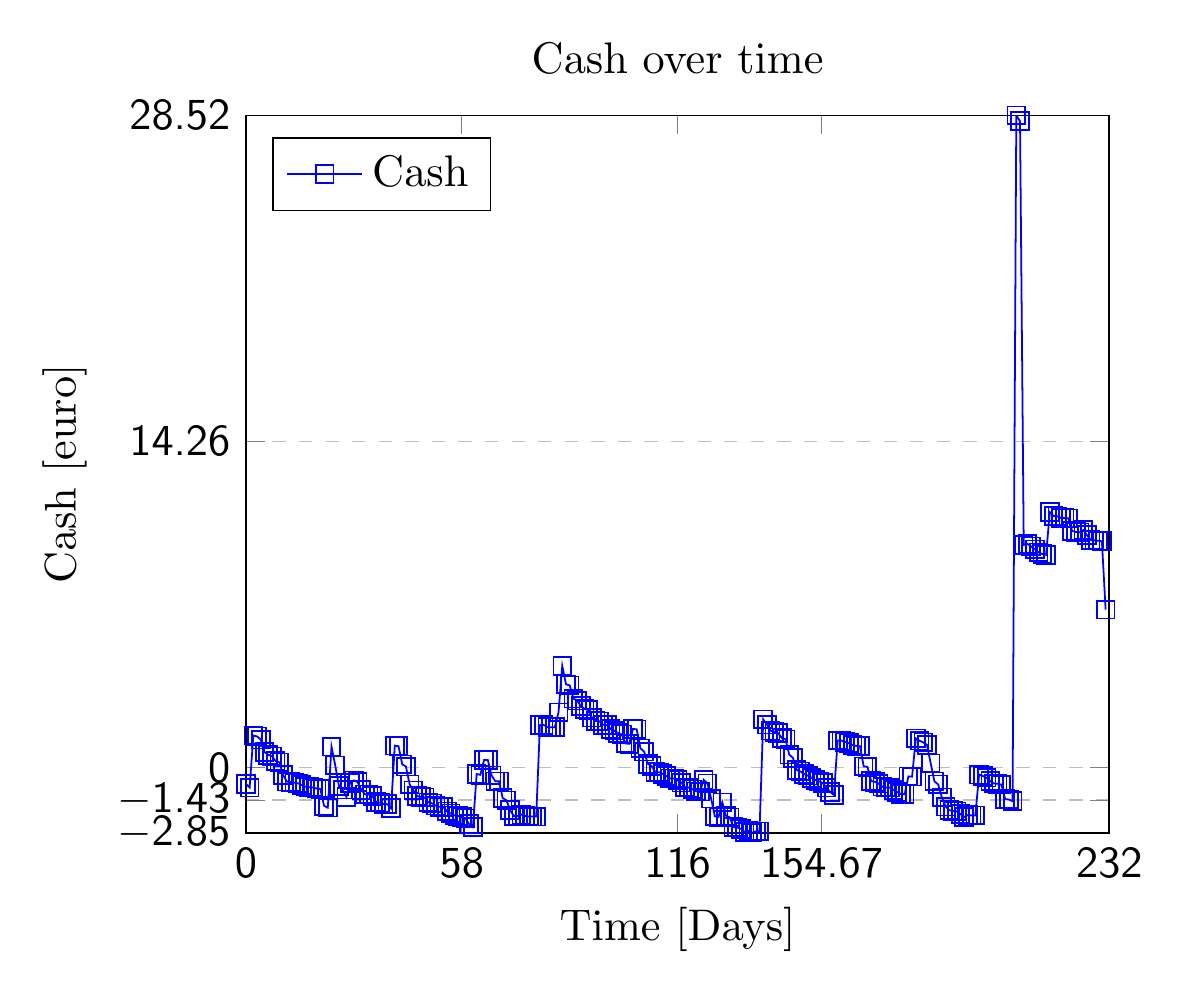
\begin{tikzpicture}[thick, scale=1.6]
\begin{axis}[
title={Cash over time},
xlabel={Time [Days]},
ylabel={Cash [euro]},
xmin=0,xmax=232,
ymin=-2.851,ymax=28.519,
xtick={0,58,116,154.666666666667,232},
ytick={-2.851,-1.4255,0,14.2595,28.519},
legend pos=north west,
ymajorgrids=true,
grid style=dashed,
]
\addplot[
color=blue,
mark=square,
]
coordinates {
(0,-0.713)(1,-0.878)(2,1.4)(3,1.36)(4,1.223)(5,0.676)(6,0.557)(7,0.49)(8,0.285)(9,0.224)(10,-0.329)(11,-0.615)(12,-0.633)(13,-0.658)(14,-0.693)(15,-0.763)(16,-0.841)(17,-0.861)(18,-0.875)(19,-0.918)(20,-0.938)(21,-1.673)(22,-1.757)(23,0.91)(24,0.094)(25,-0.81)(26,-0.968)(27,-1.29)(28,-0.668)(29,-0.563)(30,-0.637)(31,-0.976)(32,-1.175)(33,-1.175)(34,-1.255)(35,-1.51)(36,-1.534)(37,-1.594)(38,-1.603)(39,-1.78)(40,0.959)(41,0.932)(42,0.141)(43,0.04)(44,-0.738)(45,-0.996)(46,-1.25)(47,-1.286)(48,-1.309)(49,-1.52)(50,-1.564)(51,-1.664)(52,-1.719)(53,-1.719)(54,-1.913)(55,-2.009)(56,-2.089)(57,-2.114)(58,-2.164)(59,-2.224)(60,-2.478)(61,-2.605)(62,-0.287)(63,-0.32)(64,0.33)(65,0.33)(66,-0.34)(67,-0.602)(68,-0.606)(69,-1.337)(70,-1.435)(71,-1.858)(72,-2.126)(73,-2.124)(74,-2.06)(75,-2.118)(76,-2.141)(77,-2.147)(78,-2.147)(79,1.853)(80,1.863)(81,1.771)(82,1.757)(83,1.762)(84,2.412)(85,4.446)(86,3.641)(87,3.592)(88,3.015)(89,2.927)(90,2.688)(91,2.568)(92,2.508)(93,2.183)(94,2.039)(95,2.019)(96,1.869)(97,1.849)(98,1.691)(99,1.611)(100,1.51)(101,1.446)(102,1.051)(103,1.036)(104,1.686)(105,1.67)(106,0.841)(107,0.695)(108,0.162)(109,0.067)(110,-0.191)(111,-0.207)(112,-0.28)(113,-0.376)(114,-0.476)(115,-0.476)(116,-0.556)(117,-0.66)(118,-0.867)(119,-0.879)(120,-0.954)(121,-1.04)(122,-1.058)(123,-0.537)(124,-0.688)(125,-1.358)(126,-2.133)(127,-2.161)(128,-1.519)(129,-2.108)(130,-2.176)(131,-2.609)(132,-2.619)(133,-2.679)(134,-2.815)(135,-2.769)(136,-2.851)(137,-2.793)(138,-2.793)(139,2.107)(140,1.873)(141,1.608)(142,1.562)(143,1.501)(144,1.297)(145,1.236)(146,0.563)(147,0.419)(148,-0.11)(149,-0.172)(150,-0.283)(151,-0.359)(152,-0.449)(153,-0.539)(154,-0.601)(155,-0.681)(156,-0.882)(157,-1.071)(158,-1.204)(159,1.181)(160,1.18)(161,1.115)(162,1.064)(163,0.984)(164,0.942)(165,0.933)(166,0.049)(167,0.033)(168,-0.594)(169,-0.624)(170,-0.704)(171,-0.836)(172,-0.871)(173,-0.876)(174,-0.982)(175,-1.075)(176,-1.159)(177,-1.167)(178,-0.389)(179,-0.399)(180,1.273)(181,1.173)(182,1.097)(183,0.991)(184,0.185)(185,-0.604)(186,-0.739)(187,-1.3)(188,-1.709)(189,-1.867)(190,-1.9)(191,-1.918)(192,-2.039)(193,-2.17)(194,-2.079)(195,-2.094)(196,-2.094)(197,-0.31)(198,-0.37)(199,-0.447)(200,-0.599)(201,-0.7)(202,-0.712)(203,-0.748)(204,-1.382)(205,-1.4)(206,-1.473)(207,28.519)(208,28.263)(209,9.736)(210,9.779)(211,9.669)(212,9.538)(213,9.409)(214,9.336)(215,9.302)(216,11.165)(217,11.005)(218,10.987)(219,10.917)(220,10.906)(221,10.901)(222,10.349)(223,10.301)(224,10.284)(225,10.383)(226,10.158)(227,9.954)(228,9.934)(229,9.917)(230,9.896)(231,6.905)
};
\legend{Cash}
\end{axis}
\end{tikzpicture}

%Checklists.tex:%\includegraphics[scale=0.5]{stockchart.pdf}}

%\subsubsection{Cash curve from Scilab man!}
%\includegraphics[scale=0.6]{Scilab-cashBalance.png}

\end{document}

